% Section content template for individual Educative lessons
% This file contains the actual content for a specific section
% Generated from Educative API section content

% Section: Getting Ready: The Chess Game
% Section ID: 5572728729108480
% Section Slug: getting-ready-the-chess-game
% Generated: 2025-12-12T16:10:10.160823

\subsection{Problem definition}\label{GdBbXiDwBbAsUwxqCLfX8}
\\
\textbf{Chess} is a strategy board game for two players on a checkered board of 64 squares in an 8x8 grid. Each player starts with 16 pieces: one king, one queen, two rooks, two knights, two bishops, and eight pawns. The goal is to checkmate the opponent's king---this occurs when the king is in a position to be captured (\textbf{check}) and there is no way to move the king out of capture (\textbf{checkmate}).
\\
Each piece has its unique movements. The rook can move horizontally or vertically, the knight can move in an L-shape position, the bishop can move diagonally, the queen can move in any direction, and the king can move one square in any direction. Pawns have the most complex movement rules: they can move forward one square, capture diagonally, and are subject to special rules such as a two-square advance on their first move, \textbf{en passant}, and \textbf{promotion}. Most pieces, except for the knight, cannot move through or over others. The game also includes special rules, such as \textbf{castling} for the king and the rook.
\\
A chess game can end in a win, a loss, or a draw. Draws can result from stalemate, threefold repetition, the 50-move rule, insufficient material, mutual agreement, or other scenarios like resignation and forfeiture.
\\
In this LLD interview case study, you'll focus on:

\begin{itemize}
\item
\protect\phantomsection\label{zDQMKng27DMNoKw2lmOq9}
Digitally modeling the rules, state, and movements of chess pieces on a virtual board, including special rules such as castling, en passant, and pawn promotion.
\item
\protect\phantomsection\label{lKAn13Xt9V1r1k1W6cM7m}
Implementing turn-based gameplay, including legal moves, checks, checkmates, and various types of draws.
\item
\protect\phantomsection\label{NmwK1WBkHTISI7adi9z4L}
Handling edge cases such as stalemate, threefold repetition, insufficient material, resignation, and forfeiture.
\item
\protect\phantomsection\label{38IWX9DdnGqaeMMjUzPYg}
The system will keep a complete record of all moves made during the game.
\item
\protect\phantomsection\label{rKrFf-mzQlZ1Gx5UerkBG}
Players cannot retract or undo moves once played.
\end{itemize}
\\
\textbf{Note:} Numerous variations of the game of chess are played globally. In this design problem, we'll create a digital version of the standard two-player chess game, faithfully implementing the official rules and recognized situations.

\begin{figure}[htbp]
 \centering
 \begin{subfigure}[b]{0.48\textwidth}
 \centering
 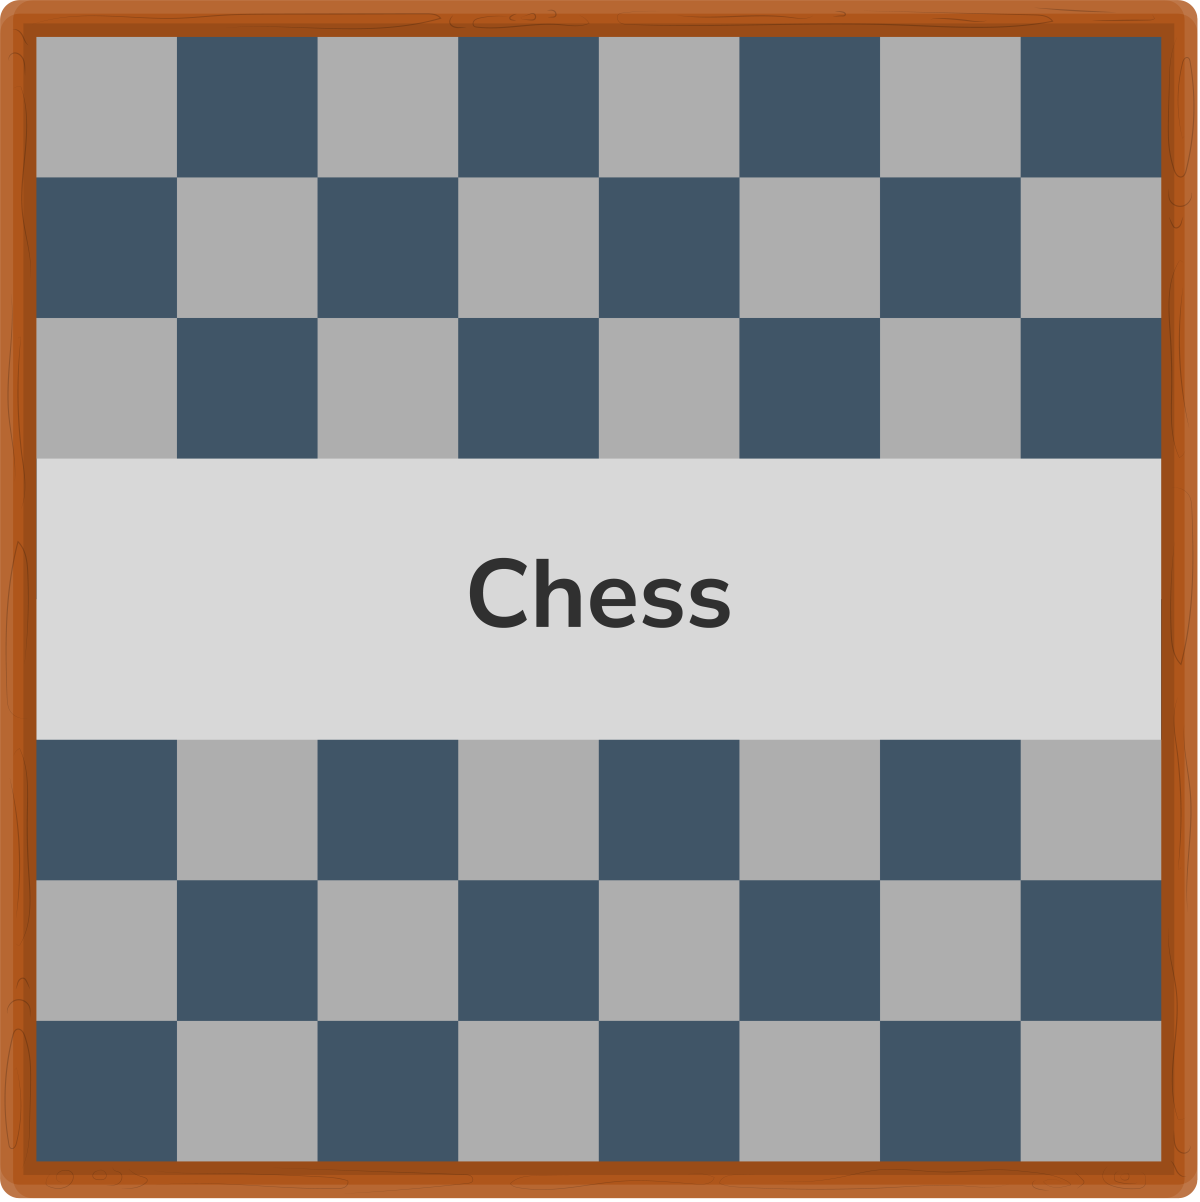
\includegraphics[width=\textwidth]{Images/chapter_17/section_5572728729108480/5703725038698496.png}
 \caption{An online chess game}
 \end{subfigure}
 \hfill
 \begin{subfigure}[b]{0.48\textwidth}
 \centering
 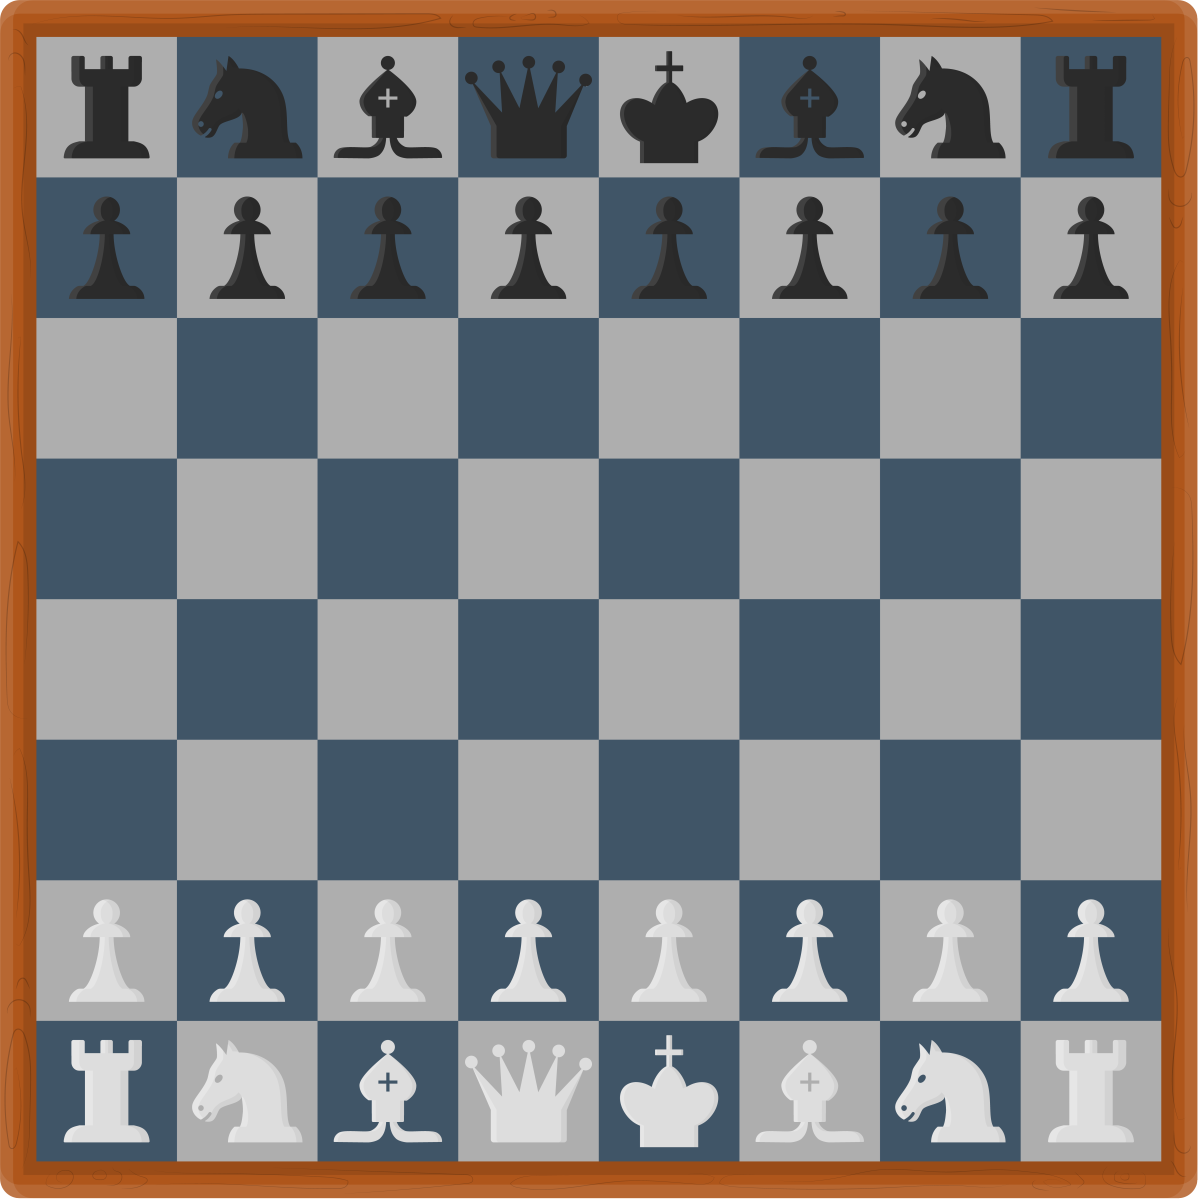
\includegraphics[width=\textwidth]{Images/chapter_17/section_5572728729108480/5986857503686656.png}
 \caption{The initial state of the chessboard before starting the game}
 \end{subfigure}
\end{figure}

\begin{figure}[htbp]
 \centering
 \begin{subfigure}[b]{0.48\textwidth}
 \centering
 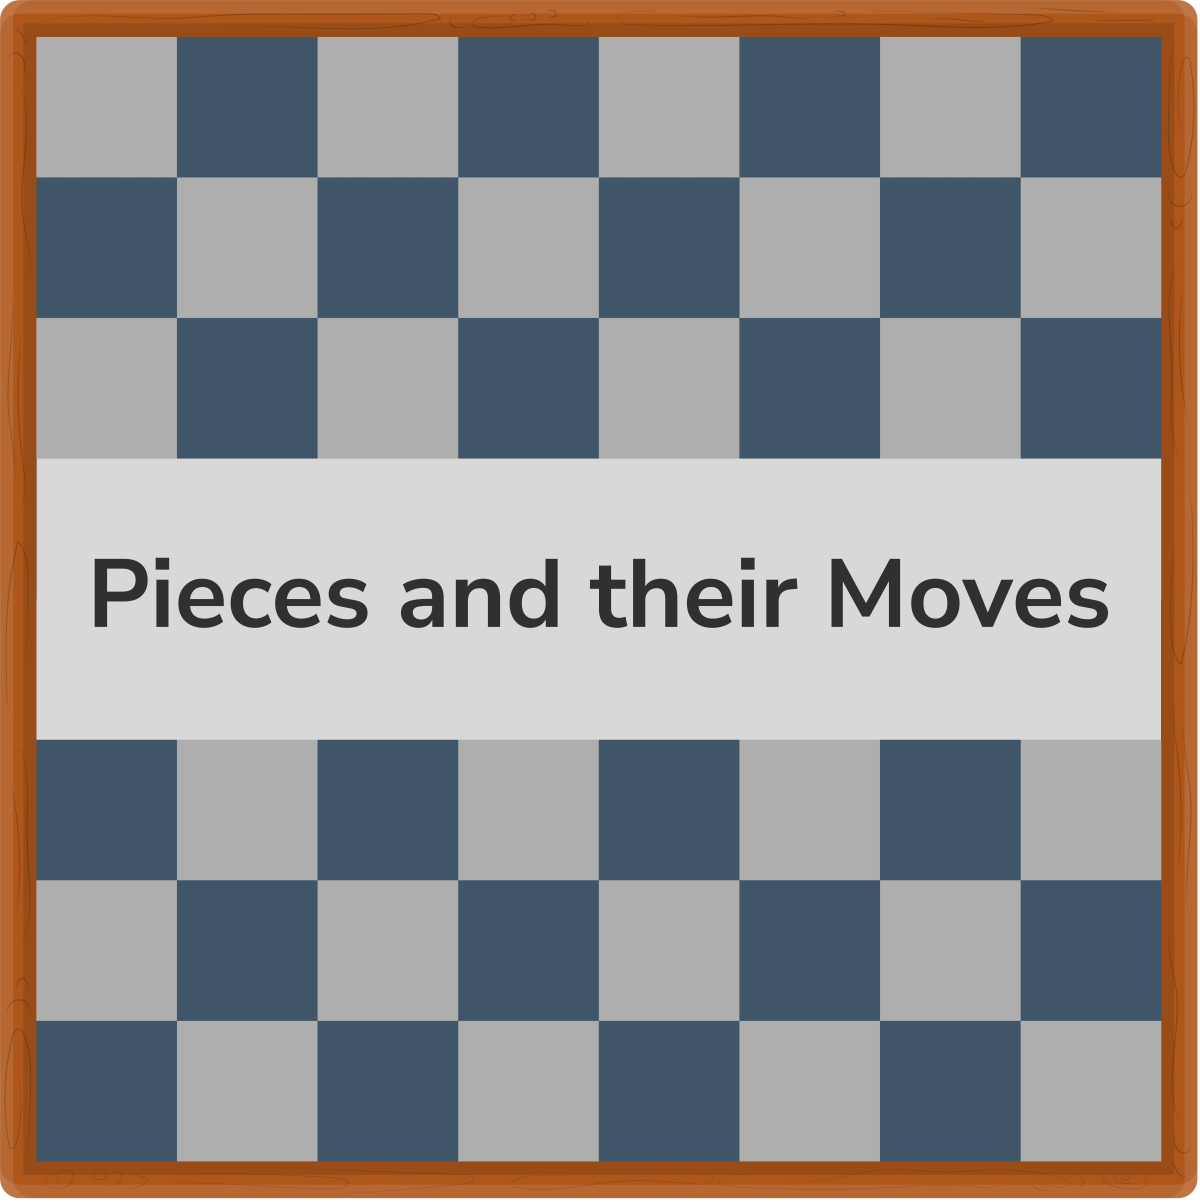
\includegraphics[width=\textwidth]{Images/chapter_17/section_5572728729108480/4888821666938880.png}
 \caption{Chess pieces and their moves}
 \end{subfigure}
 \hfill
 \begin{subfigure}[b]{0.48\textwidth}
 \centering
 
\includegraphics[width=\textwidth]{Images/chapter_17/section_5572728729108480/5360069639405568.png}
 \caption{The “king” piece and its moves}
 \end{subfigure}
\end{figure}

\begin{figure}[htbp]
 \centering
 \begin{subfigure}[b]{0.48\textwidth}
 \centering
 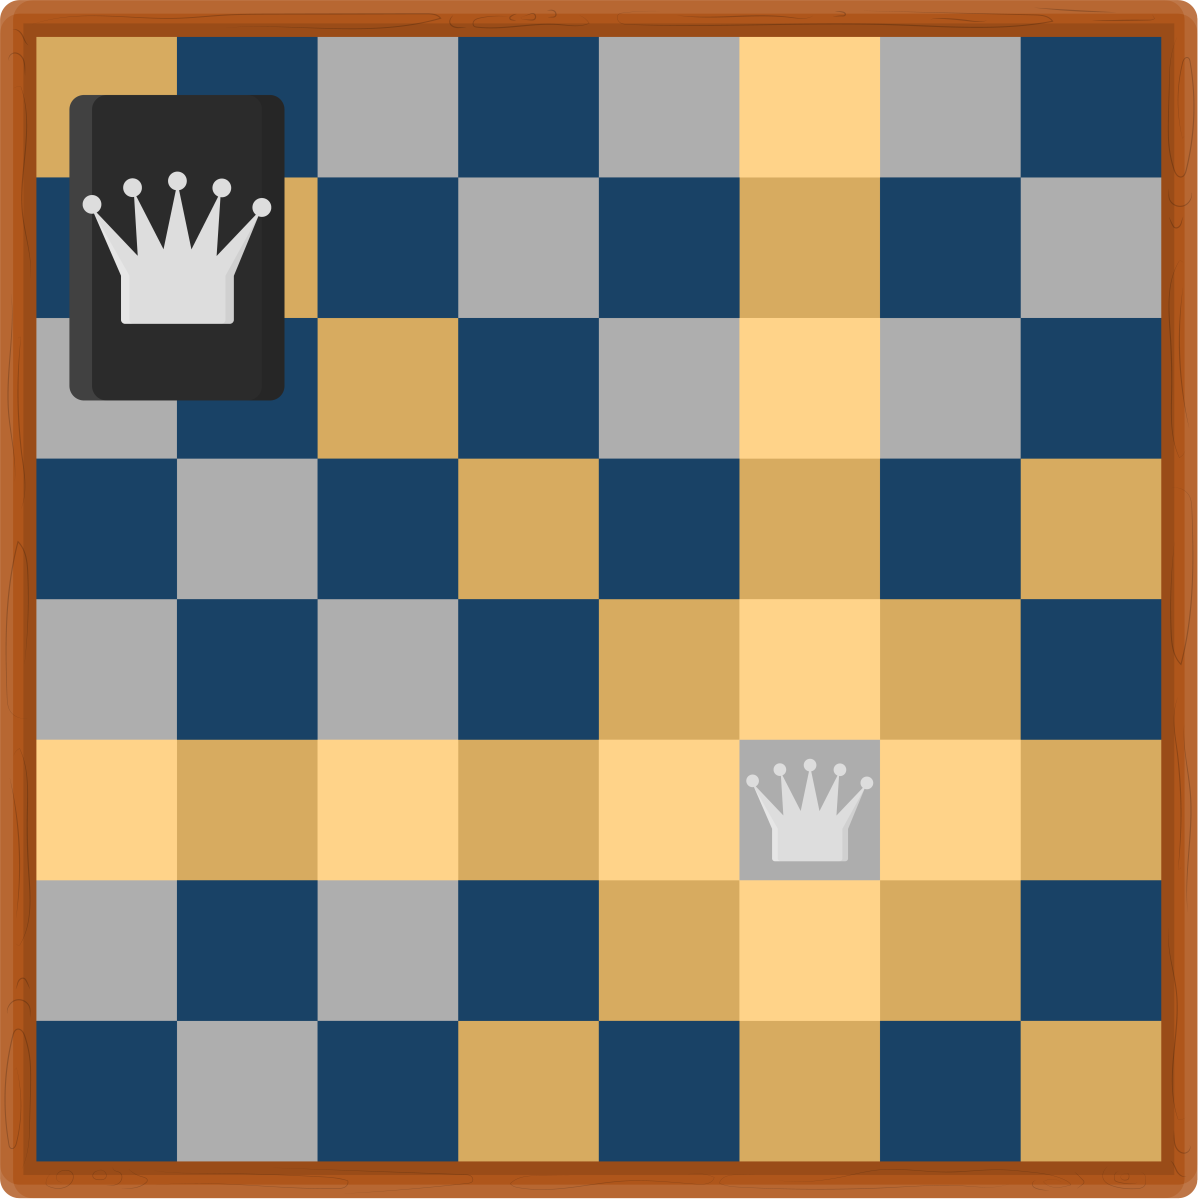
\includegraphics[width=\textwidth]{Images/chapter_17/section_5572728729108480/5902972598091776.png}
 \caption{The “queen” piece and its moves}
 \end{subfigure}
 \hfill
 \begin{subfigure}[b]{0.48\textwidth}
 \centering
 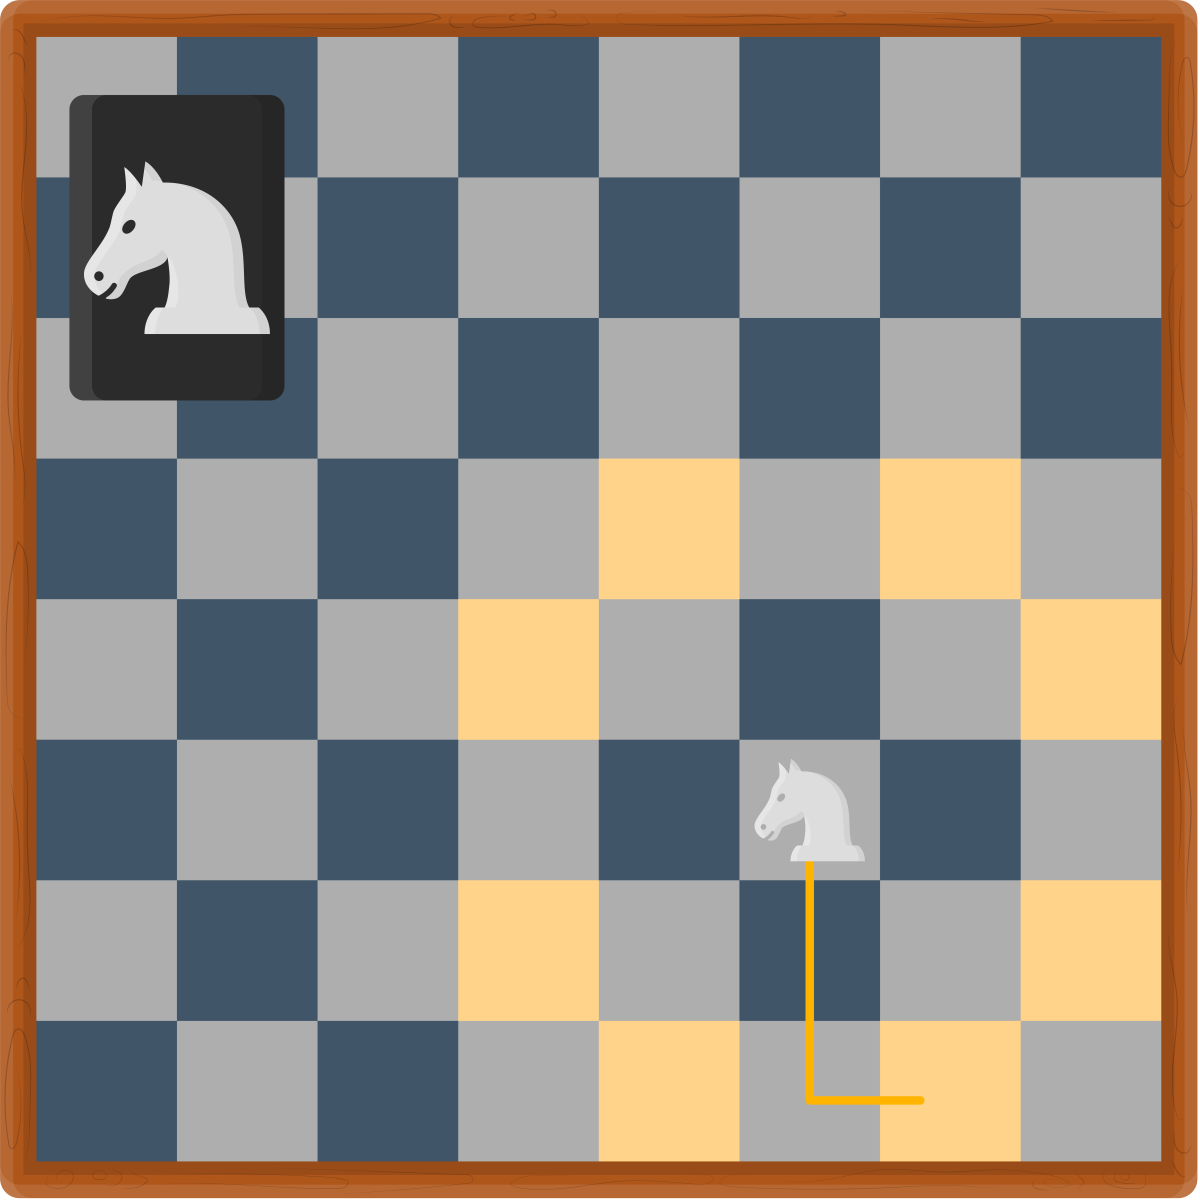
\includegraphics[width=\textwidth]{Images/chapter_17/section_5572728729108480/4745041865342976.png}
 \caption{The “knight” piece and its moves}
 \end{subfigure}
\end{figure}

\begin{figure}[htbp]
 \centering
 \begin{subfigure}[b]{0.48\textwidth}
 \centering
 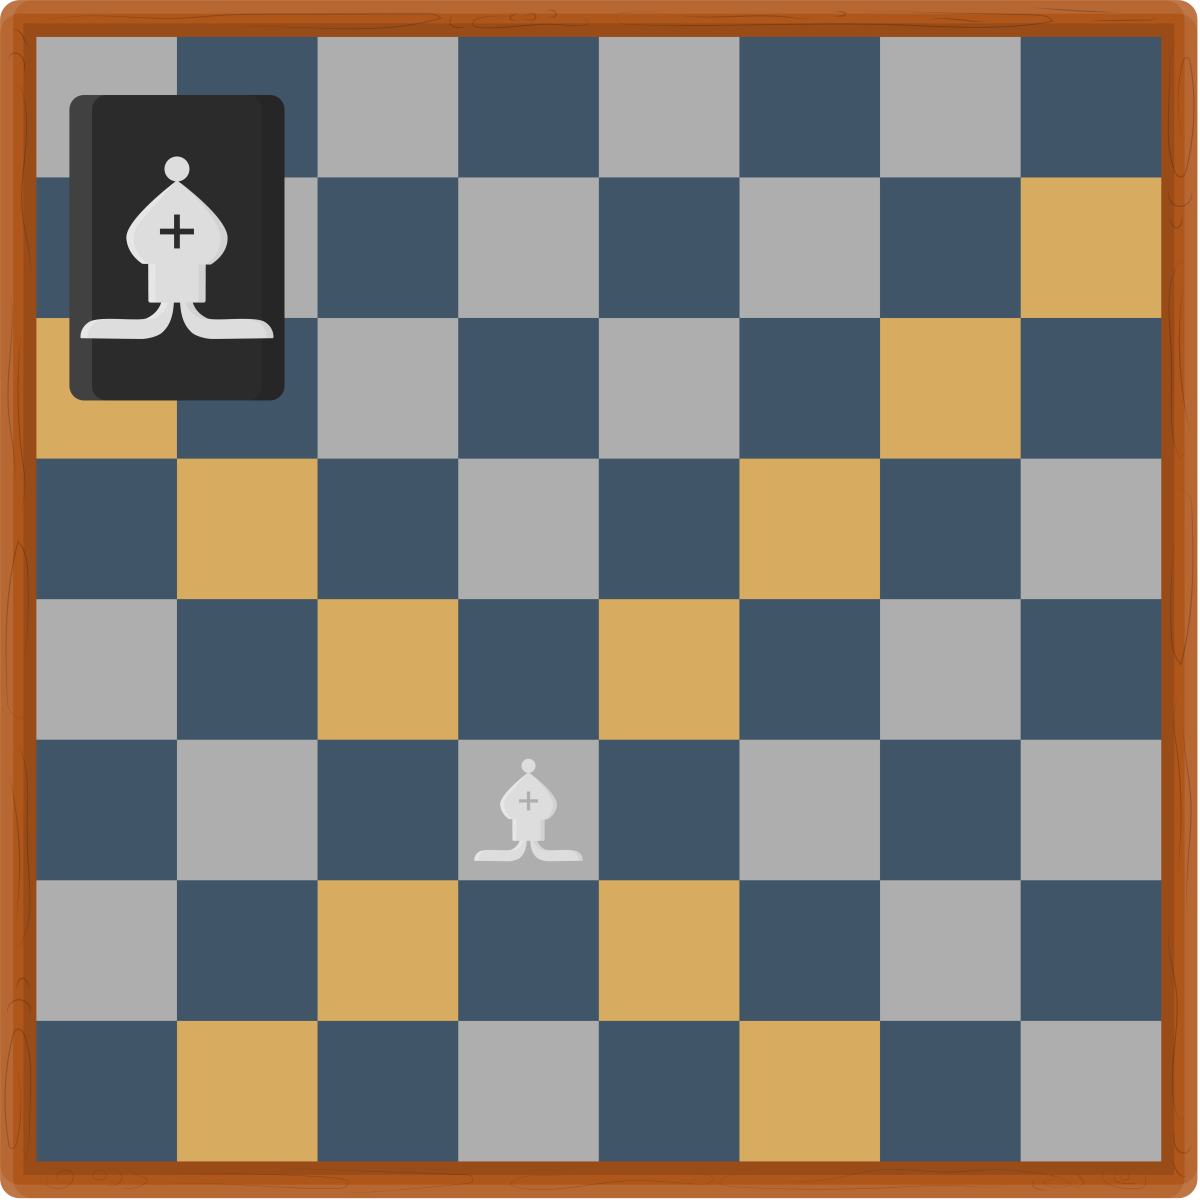
\includegraphics[width=\textwidth]{Images/chapter_17/section_5572728729108480/4621873343365120.png}
 \caption{The “bishop” piece and its moves}
 \end{subfigure}
 \hfill
 \begin{subfigure}[b]{0.48\textwidth}
 \centering
 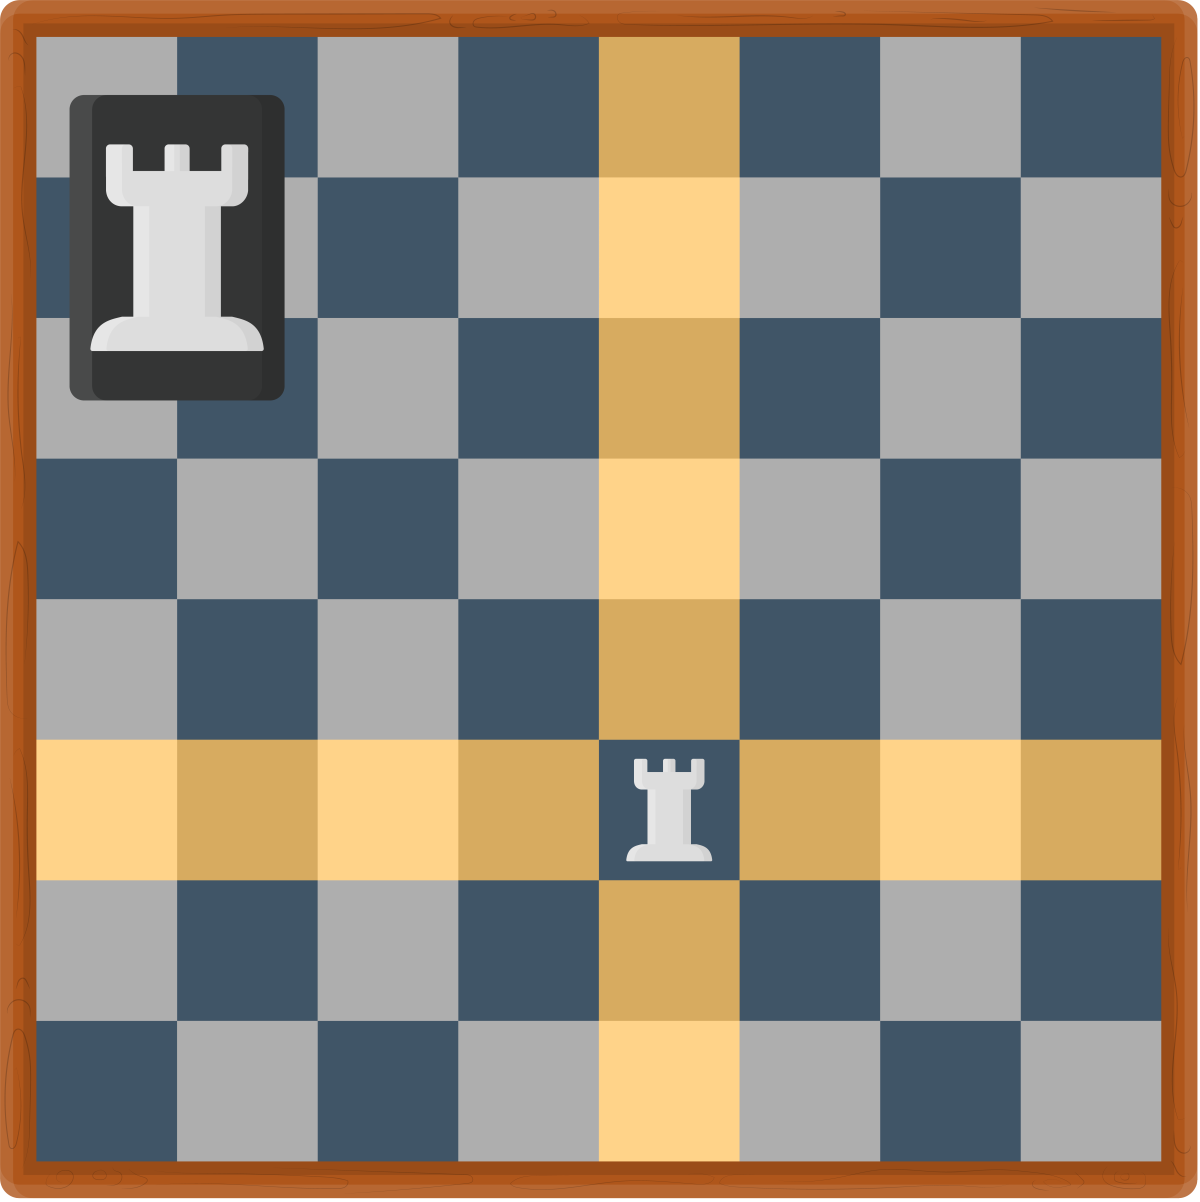
\includegraphics[width=\textwidth]{Images/chapter_17/section_5572728729108480/5042135557734400.png}
 \caption{The “rook” piece and its moves}
 \end{subfigure}
\end{figure}

\begin{figure}[htbp]
 \centering
 \begin{subfigure}[b]{0.48\textwidth}
 \centering
 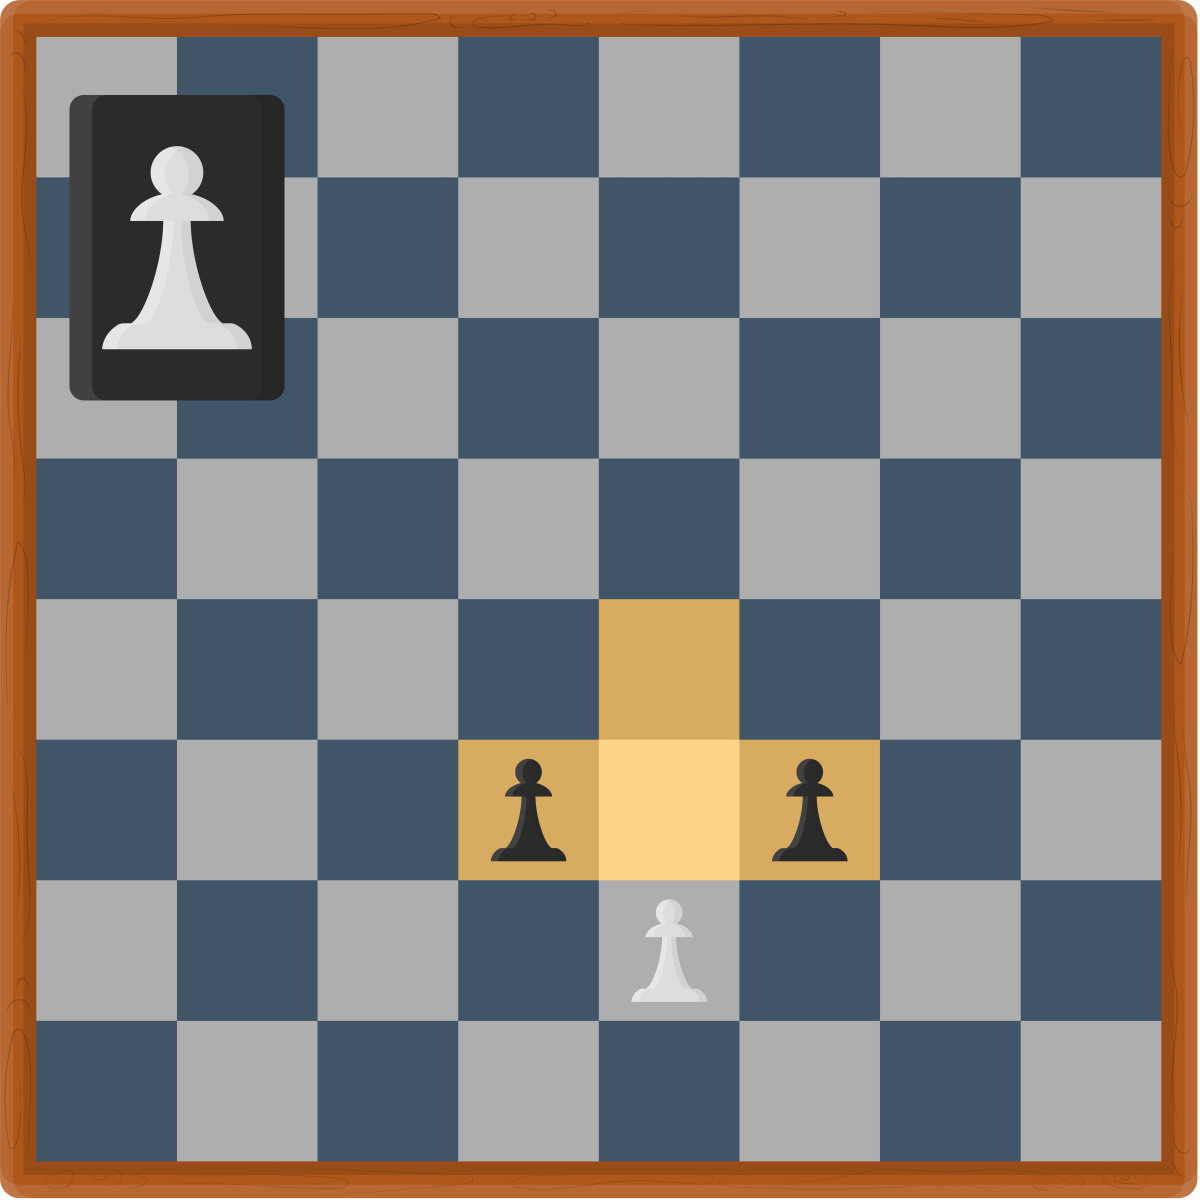
\includegraphics[width=\textwidth]{Images/chapter_17/section_5572728729108480/6333395765559296.png}
 \caption{The “pawn” piece and its moves}
 \end{subfigure}
 \hfill
 \begin{subfigure}[b]{0.48\textwidth}
 \centering
 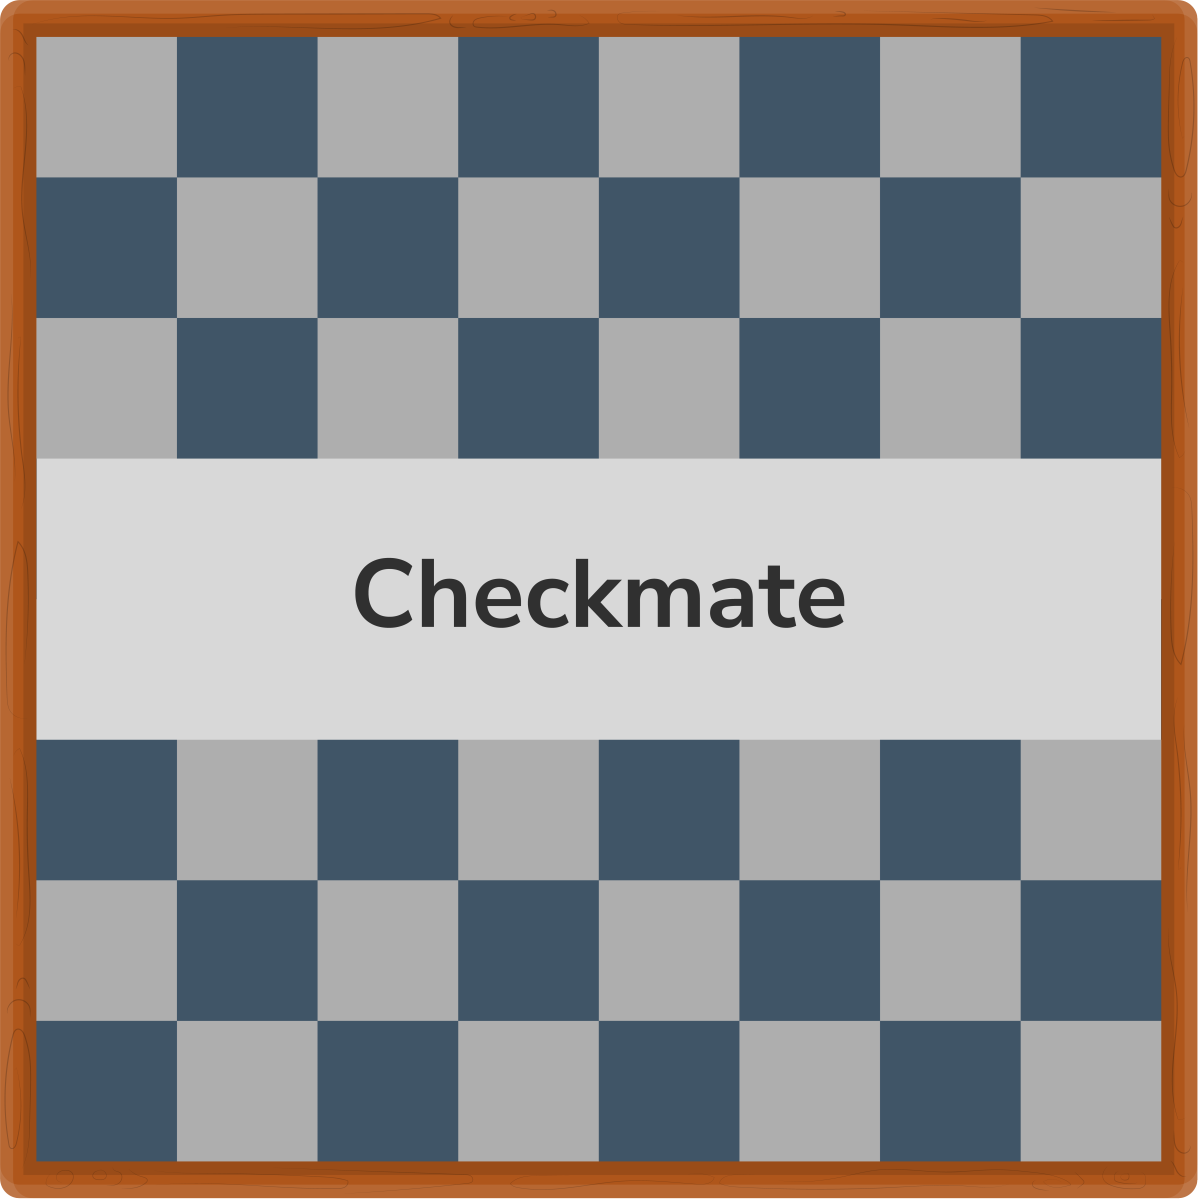
\includegraphics[width=\textwidth]{Images/chapter_17/section_5572728729108480/4735461320032256.png}
 \caption{Checkmate in the game}
 \end{subfigure}
\end{figure}

\begin{figure}[htbp]
 \centering
 \begin{subfigure}[b]{0.48\textwidth}
 \centering
 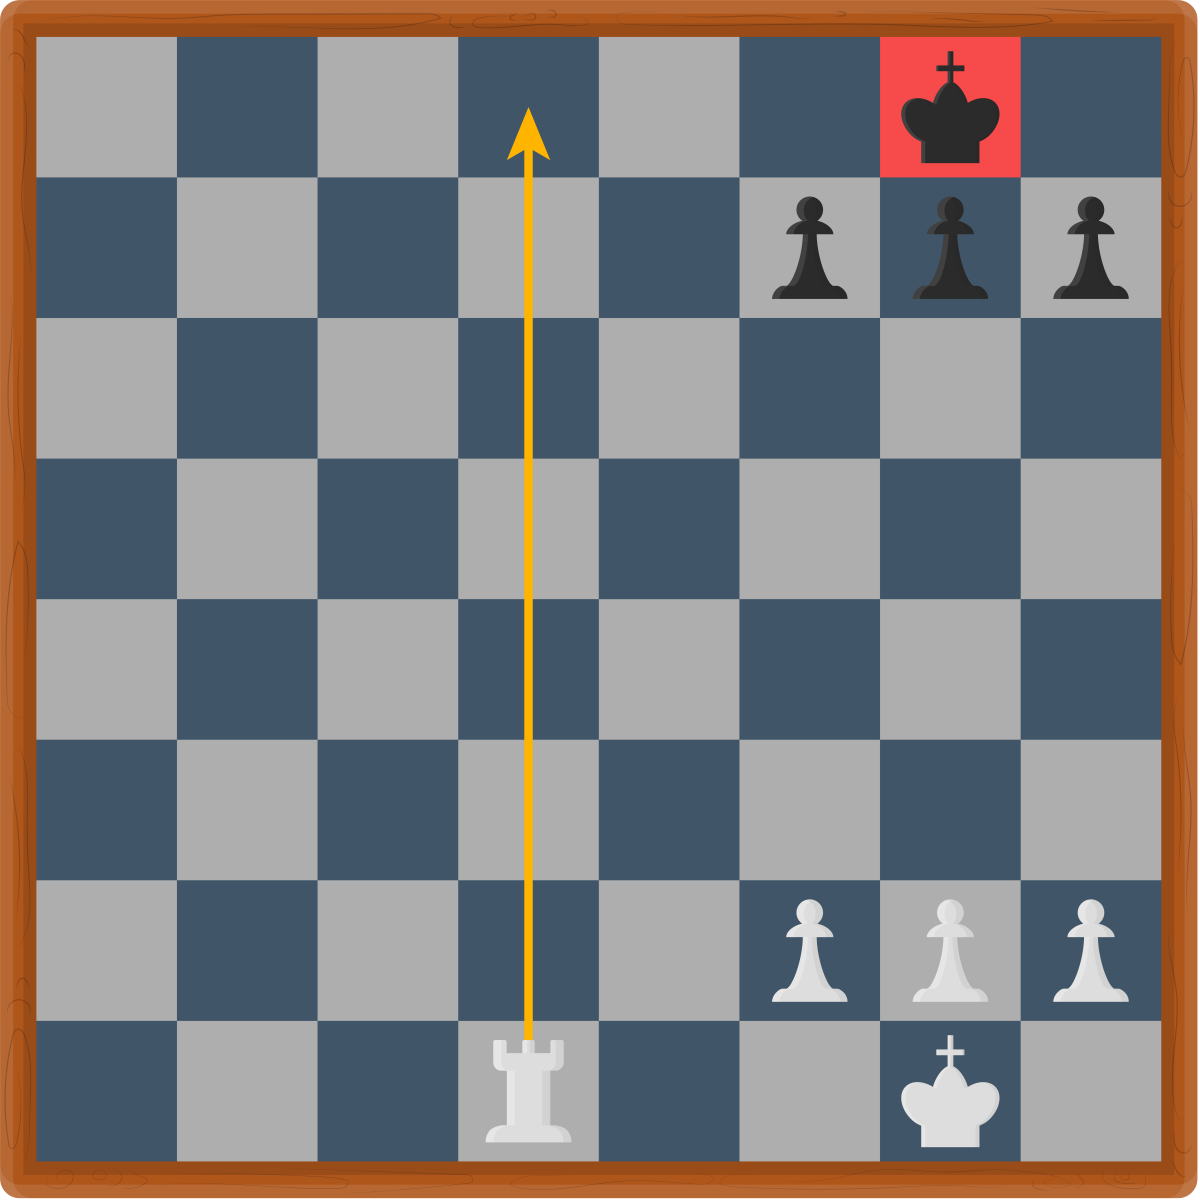
\includegraphics[width=\textwidth]{Images/chapter_17/section_5572728729108480/6084973145882624.png}
 \caption{Demonstration of a scenario where a checkmate has occurred}
 \end{subfigure}
\end{figure}

\subsection{Expectations from the interviewee}\label{3pZ0V0TX6jB71x2_DAAtL}
\\
There are several components in a chess game, each with specific constraints and requirements. The following provides an overview of some of the main expectations that the interviewer will want to hear you discuss in more detail during the interview.

\subsubsection{Chess pieces}\label{gPS6TUwl2cvcfAz8lu2Jh}
\\
The chess pieces have their own specifications according to the game's rules that need to be clarified by the interviewer. Therefore, you may ask the following questions:

\begin{enumerate}
\item
\protect\phantomsection\label{OGcsdcVguY4VySnMiKL2U}
How many chess pieces are there in the game?
\item
\protect\phantomsection\label{Upn_ptB_5TJc9Ec_1gKg3}
What are the different chess pieces, and what are their respective moves?
\item
\protect\phantomsection\label{AOy66guLpze6VnIteF2ll}
Which piece is the weakest in chess?
\item
\protect\phantomsection\label{XDUifB6BRJ1ErADGZwSHN}
Which piece is the strongest in chess?
\end{enumerate}

\subsubsection{Gameplay}\label{65gA9Llm3JKPsQp5_metY}
\\
In chess, the two opposing teams try to achieve the state of checkmate to win the game, or they face some special cases, like a stalemate, that need to be clarified by the interviewer. You may ask the following questions regarding them:

\begin{enumerate}
\item
\protect\phantomsection\label{GArA5EVwv8QbR5pW21VRB}
Which player takes the first turn?
\item
\protect\phantomsection\label{V7vJxQhl2UsIRlkNRVvoY}
What are the rules of the game?
\item
\protect\phantomsection\label{BX31--glOLD9_jWu2YAgl}
What is a checkmate?
\item
\protect\phantomsection\label{4pZU8UxKJJkYGxOOsPqr8}
How does a stalemate happen?
\item
\protect\phantomsection\label{Yq1YN5Z_wougIlwWlW_vK}
Can a player forfeit/resign from the game?
\end{enumerate}

\subsection{Design approach}\label{IaKKBorxmgqQpfrscU7Zo}
\\
We will design this chess game system using a bottom-up approach. For this purpose, we will follow these steps:

\begin{itemize}
\item
\protect\phantomsection\label{cqs1Io1erPWIAu1CHwTrP}
First, we'll define the core entities: \texttt{ChessPiece}, \texttt{BoardSquare}, and \texttt{Player}.
\item
\protect\phantomsection\label{U9Yy0WNcAe7fZl50kjqHC}
Next, we'll model composite components like \texttt{ChessBoard}, \texttt{Move}, and \texttt{Game}, capturing piece movement, board state, and game progression.
\item
\protect\phantomsection\label{qGc4U5I8P61weUYiD-kBP}
We'll ensure the design supports the enforcement of chess rules, detection of check, checkmate, and draw conditions, and handles move validation and player interactions.
\item
\protect\phantomsection\label{OpcMlGXbe8jmdWAjjn5O6}
The system will be scalable for future extensions such as move history, undo/redo, and online multiplayer features.
\end{itemize}
\\
This design approach will address edge cases and adhere to SOLID principles, making the system easy to extend, maintain, and test. Diagrams and code will illustrate major workflows and class structures.

\subsection{Design pattern~}\label{CmVqJxULuf2M9UtshDr-H}
\\
During an interview, discussing the design patterns that the chess game falls under is always a good practice. Stating the design patterns gives the interviewer a positive impression and shows that the interviewee is well-versed in the advanced concepts of object-oriented design.
\\
Try to answer the following question. If you are not familiar with design patterns, don't worry! You can learn about them by asking, ``Define design patterns.''
\\
Try to answer the following question. If you are not familiar with design patterns, don't worry! You can learn about them by asking questions like, ``Define design patterns.''

\textbf{Question:}

Which design pattern(s) should be used to design a Chess game? Please elaborate on your choice(s).

Let's explore the requirements of the online chess game in the next lesson.

% End of section content